\chapter{Appendix}
\label{chap:appendix}

\section{Embedded Project Evidence}
\label{app:evidence}

The artifacts in Table~\ref{tab:evidence-artifacts} are embedded in the thesis as attachments where possible. The appendix excludes working-only research notes, the internal canonical specification, template documents, AVIF sample images, the larger image-test dataset, and PlantUML source files. The rendered diagrams are included because they are the thesis-ready versions of the diagram sources.

\begin{table}[htbp]
\small
\centering
\begin{tabularx}{\textwidth}{P{0.26\textwidth}P{0.20\textwidth}Y}
\toprule
Artifact & Attachment & Evidence use \\
\midrule
Buy2Sell project overview & \attachfile[description={Buy2Sell project overview}]{artifacts/buy2sell-project-overview.pdf} & External project brief describing manual registration, label fields, OCR and barcode idea, and expected value. \\
Project proposal & \attachfile[description={English SE BSc proposal}]{artifacts/english-se-bsc-rev2.pdf} & Proposal, tone reference, sprint framing, and planning references for OCR and text recognition options. \\
Meeting notes & \attachfile[description={Meeting notes 2026-02-23}]{artifacts/meeting-notes-2026-02-23.pdf} & Notes from the project meeting, including scope, fields, multiple images, remote/local processing, and prototype goals. \\
Requirements register & \attachfile[description={Project requirements register}]{artifacts/project-requirements.pdf} & Full requirement register with requirement IDs, acceptance criteria, scope, verification method, and delivery phase. \\
Gantt chart & \attachfile[description={Gantt chart}]{artifacts/gantt-chart.pdf} & Project schedule and planning timeline. \\
Figma design & \attachfile[description={Figma design}]{artifacts/figma-design.pdf} & Design artifact showing intended capture, validation, history, queue, and configuration surfaces. \\
KPI evaluation results & \attachfile[description={Anonymized KPI evaluation results}]{artifacts/kpi-anonymized.pdf} & Anonymized per-image and per-field extraction correctness evidence for the Buy2Sell image evaluation. \\
Expo app structure reference & \cite{expo-folder-structure} & Local architecture reference used when organizing screens, routes, and reusable code. \\
\bottomrule
\end{tabularx}
\caption{Local project evidence artifacts, part 1.}
\label{tab:evidence-artifacts}
\end{table}

\begin{table}[htbp]
\small
\centering
\begin{tabularx}{\textwidth}{P{0.26\textwidth}P{0.20\textwidth}Y}
\toprule
Artifact & Attachment & Evidence use \\
\midrule
System context diagram & \attachfile[description={System context diagram}]{artifacts/system-context.png} & Rendered architecture figure used in Chapter~\ref{chap:introduction}. \\
Component diagram & \attachfile[description={Component diagram}]{artifacts/component-diagram.png} & Rendered architecture figure used in Chapter~\ref{chap:design}. \\
Capture pipeline diagram & \attachfile[description={Capture pipeline diagram}]{artifacts/app-pipeline-activity.png} & Rendered activity diagram for the capture-to-ingest workflow. \\
Data model diagram & \attachfile[description={Local data model diagram}]{artifacts/local-persistence-model.png} & Rendered local data model figure. \\
User-flow diagram & \attachfile[description={User-flow diagram}]{artifacts/ui-flow.png} & Rendered user-flow figure. \\
State model diagram & \attachfile[description={Attempt state model diagram}]{artifacts/app-state-machine.png} & Rendered attempt state model. \\
Extraction sequence diagram & \attachfile[description={Extraction sequence diagram}]{artifacts/extraction-pipeline-sequence.png} & Rendered extraction sequence diagram. \\
Provider router diagram & \attachfile[description={Provider router diagram}]{artifacts/provider-router-logic.png} & Rendered provider-routing logic diagram. \\
Domain model diagram & \attachfile[description={Domain model diagram}]{artifacts/domain-model.png} & Rendered domain model diagram. \\
Ingest pipeline diagram & \attachfile[description={Ingest pipeline diagram}]{artifacts/ingest-pipeline-sequence.png} & Rendered ingest sequence diagram. \\
Wireframes & \attachfile[description={Capture wireframe}]{artifacts/wireframe-capture.png} \attachfile[description={Confirm wireframe}]{artifacts/wireframe-confirm-edit.png} \attachfile[description={History wireframe}]{artifacts/wireframe-history.png} \attachfile[description={Settings wireframe}]{artifacts/wireframe-settings.png} & Rendered UI wireframes for the main application surfaces. \\
\bottomrule
\end{tabularx}
\caption{Local project evidence artifacts, part 2.}
\end{table}

\section{KPI Evaluation Evidence}
\label{app:kpi-evidence}

The KPI evidence artifact contains anonymized image identifiers, scored field counts, field-level correctness values, exact-match flags, semantic adjudication flags, and discrepancy notes. The artifact excludes the original Buy2Sell label images and uses anonymized identifiers so that the evaluation can be inspected without exposing NDA-protected image content.

\section{Lighthouse Evidence}
\label{app:lighthouse}

The Lighthouse reports are embedded as attachments and included as appendix pages. They were captured against the web routes for Capture, Confirm, History, and Settings. Their performance scores should be interpreted as development-mode evidence, not production performance measurements.

\begin{table}[htbp]
\centering
\begin{tabularx}{\textwidth}{>{\raggedright\arraybackslash}p{0.25\textwidth}>{\raggedright\arraybackslash}p{0.25\textwidth}X}
\toprule
Route & Attachment & Evidence use \\
\midrule
Capture & \attachfile[description={Lighthouse Capture}]{artifacts/lighthouse-capture.pdf} & Route inspection for the capture workflow. \\
Confirm and Edit & \attachfile[description={Lighthouse Confirm}]{artifacts/lighthouse-confirm.pdf} & Route inspection for the review and editing workflow. \\
History & \attachfile[description={Lighthouse History}]{artifacts/lighthouse-history.pdf} & Route inspection for attempt traceability. \\
Settings & \attachfile[description={Lighthouse Settings}]{artifacts/lighthouse-settings.pdf} & Route inspection for provider and ingest configuration. \\
\bottomrule
\end{tabularx}
\caption{Lighthouse evidence reports.}
\label{tab:lighthouse}
\end{table}

\section{Glossary}

\begin{table}[htbp]
\centering
\begin{tabularx}{\textwidth}{>{\raggedright\arraybackslash}p{0.25\textwidth}X}
\toprule
Term & Definition \\
\midrule
Attempt & A single capture-to-send execution record with status, metadata, and outputs. \\
Ingest & The receiving endpoint and process that accepts reviewed JSON payloads from the app. \\
Provider & A configured vision-language backend used for extraction. \\
BYOK & Bring your own key. The operator configures provider and ingest credentials for the deployment context. \\
Mode & The execution mode selected for extraction, such as remote vision-language extraction or future local vision-language extraction. \\
Unified Process & An iterative lifecycle with overlapping disciplines (requirements, design, implementation, validation) rather than one-way phase handovers. \\
MoSCoW & Requirement-priority method using Must, Should, Could, and Won't categories. \\
ORM & Object-Relational Mapping. A typed layer that maps relational tables and queries to application-level code constructs. \\
Drizzle ORM & The ORM used in this project to model SQLite tables and queries in typed TypeScript repository code. \\
VLM & Vision-language model used to map label images to structured JSON fields. \\
Schema version & Version identifier for the structured JSON contract. \\
Offline queue & Persistent FIFO queue of accepted payloads waiting for network delivery. \\
Idempotency key & Stable key derived from attempt identity to prevent duplicate ingest effects. \\
\bottomrule
\end{tabularx}
\caption{Required glossary terms.}
\label{tab:glossary}
\end{table}

\section{Risk Register}

\begin{table}[htbp]
\centering
\begin{tabularx}{\textwidth}{>{\raggedright\arraybackslash}p{0.25\textwidth}XX}
\toprule
Risk & Impact & Mitigation \\
\midrule
Provider outage or rate limit & Extraction unavailable & Provider configuration, retry logic, clear user feedback, and queue-preserving workflow. \\
Low-quality label image & Missing or incorrect fields & Human review, retry capture, barcode evidence, and schema validation. \\
Network loss during submission & Accepted payload not delivered immediately & Persistent offline queue and idempotency key. \\
Credential leakage & Unauthorized provider or ingest use & Secure storage on native platforms, redacted diagnostics, BYOK settings. \\
Schema drift & Backend cannot consume payload & Schema versioning, Zod validation, and contract tests. \\
Browser barcode support variance & Web barcode detection inconsistent & Runtime feature detection and fallback detector package. \\
\bottomrule
\end{tabularx}
\caption{Risks and mitigations.}
\label{tab:risks}
\end{table}

\section{Example JSON Payload}

The accepted ingest payload contains reviewed structured data, barcode enrichment, auxiliary text, and metadata. A simplified example is shown below.

\begin{lstlisting}[caption={Simplified accepted ingest payload},label={lst:payload}]
{
  "schema_version": "1.0",
  "attempt_id": "attempt-...",
  "accepted_revision": 1,
  "structured_json": {
    "manufacturer": "Phoenix Contact",
    "product_number": "2865463",
    "product_text": "MACX MCR-EX-SL-NAM-2T Isolation Switch Amplifier",
    "ean_or_upc": "4046356160483",
    "country_of_origin": "Germany",
    "condition": "Used",
    "quantity": 1
  },
  "enrichment": {
    "barcodes": []
  },
  "metadata": {
    "provider_id": "openai",
    "model": "...",
    "created_at": "..."
  }
}
\end{lstlisting}

\section{Automated Tests List}
\label{app:automated-tests}

The validation chapter summarizes test areas. This appendix lists the automated test files present in the repository so the evidence can be traced from the thesis to concrete checks.

\begin{table}[htbp]
\footnotesize
\centering
\begin{tabularx}{\textwidth}{P{0.22\textwidth}Y}
\toprule
Area & Test files \\
\midrule
App and API routing & \path{tests/app/page-metadata.test.tsx}, \path{tests/app/api/route-files.test.ts}, \path{tests/app/api/webfetch-proxy-api.test.ts}, \path{tests/app/api/openai-codex-proxy-api.test.ts}, \path{tests/app/api/github-copilot-proxy-api.test.ts}, \path{tests/app/api/github-copilot-oauth-api.test.ts}, \path{tests/app/api/exa-mcp-proxy-api.test.ts} \\
Remote extraction and ingest & \path{tests/api/remote-extractor.test.ts}, \path{tests/api/ingest-transport.test.ts}, \path{tests/api/providers/extraction-prompt.test.ts} \\
Services & \path{tests/services/capture-pipeline.test.ts}, \path{tests/services/gallery-import.test.ts}, \path{tests/services/image-store.test.ts}, \path{tests/services/barcode-detector-web.test.ts}, \path{tests/services/provider-catalog.test.ts}, \path{tests/services/provider-oauth.test.ts}, \path{tests/services/extraction-retry.test.ts}, \path{tests/services/manufacturer-websearch.test.ts}, \path{tests/services/queue-worker.test.ts}, \path{tests/services/queue-replay.integration.test.ts}, \path{tests/services/submission-service.test.ts}, \path{tests/services/toast-state.test.ts} \\
Repositories and storage & \path{tests/repositories/attempt-repository.test.ts}, \path{tests/repositories/queue-repository.test.ts}, \path{tests/repositories/settings-repository.test.ts}, \path{tests/repositories/settings-repository-web.test.ts}, \path{tests/db/secure-store.test.ts} \\
Types and utilities & \path{tests/types/app-error.test.ts}, \path{tests/types/item-schema.test.ts}, \path{tests/types/provider-error-normalization.test.ts}, \path{tests/types/user-feedback.test.ts}, \path{tests/utils/idempotency.test.ts}, \path{tests/utils/merge-extraction-result.test.ts}, \path{tests/utils/retry-policy.test.ts} \\
Components & \path{tests/components/accessibility.test.tsx}, \path{tests/components/button.test.tsx}, \path{tests/components/diagnostic-disclosure.test.tsx}, \path{tests/components/option-picker.test.tsx} \\
\bottomrule
\end{tabularx}
\caption{Automated tests list.}
\label{tab:automated-tests}
\end{table}

\section{Included Evidence PDF Pages}

The following pages include selected PDF artifacts directly in the thesis appendix in addition to the embedded file attachments.

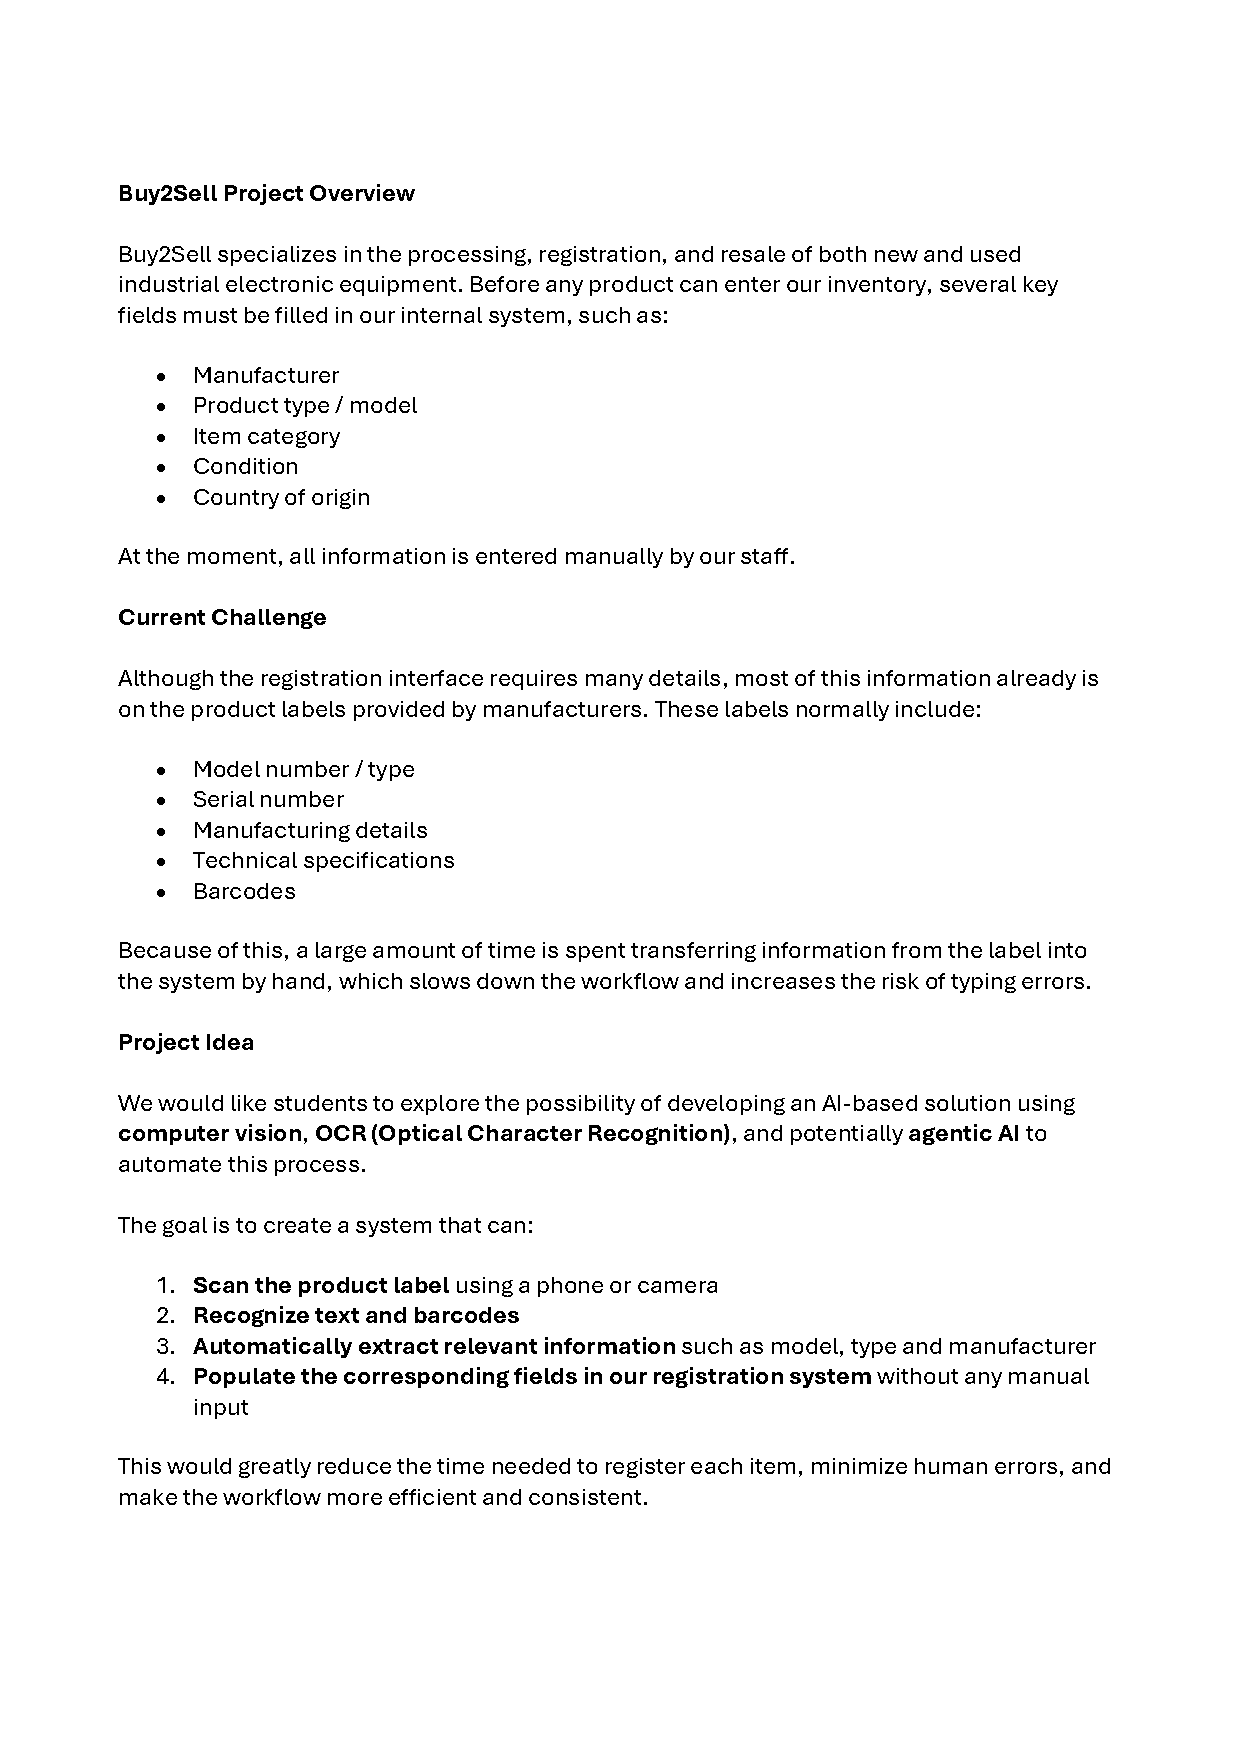
\includepdf[pages=-,pagecommand={}]{artifacts/buy2sell-project-overview.pdf}

\includepdf[pages=-,pagecommand={}]{artifacts/english-se-bsc-rev2.pdf}
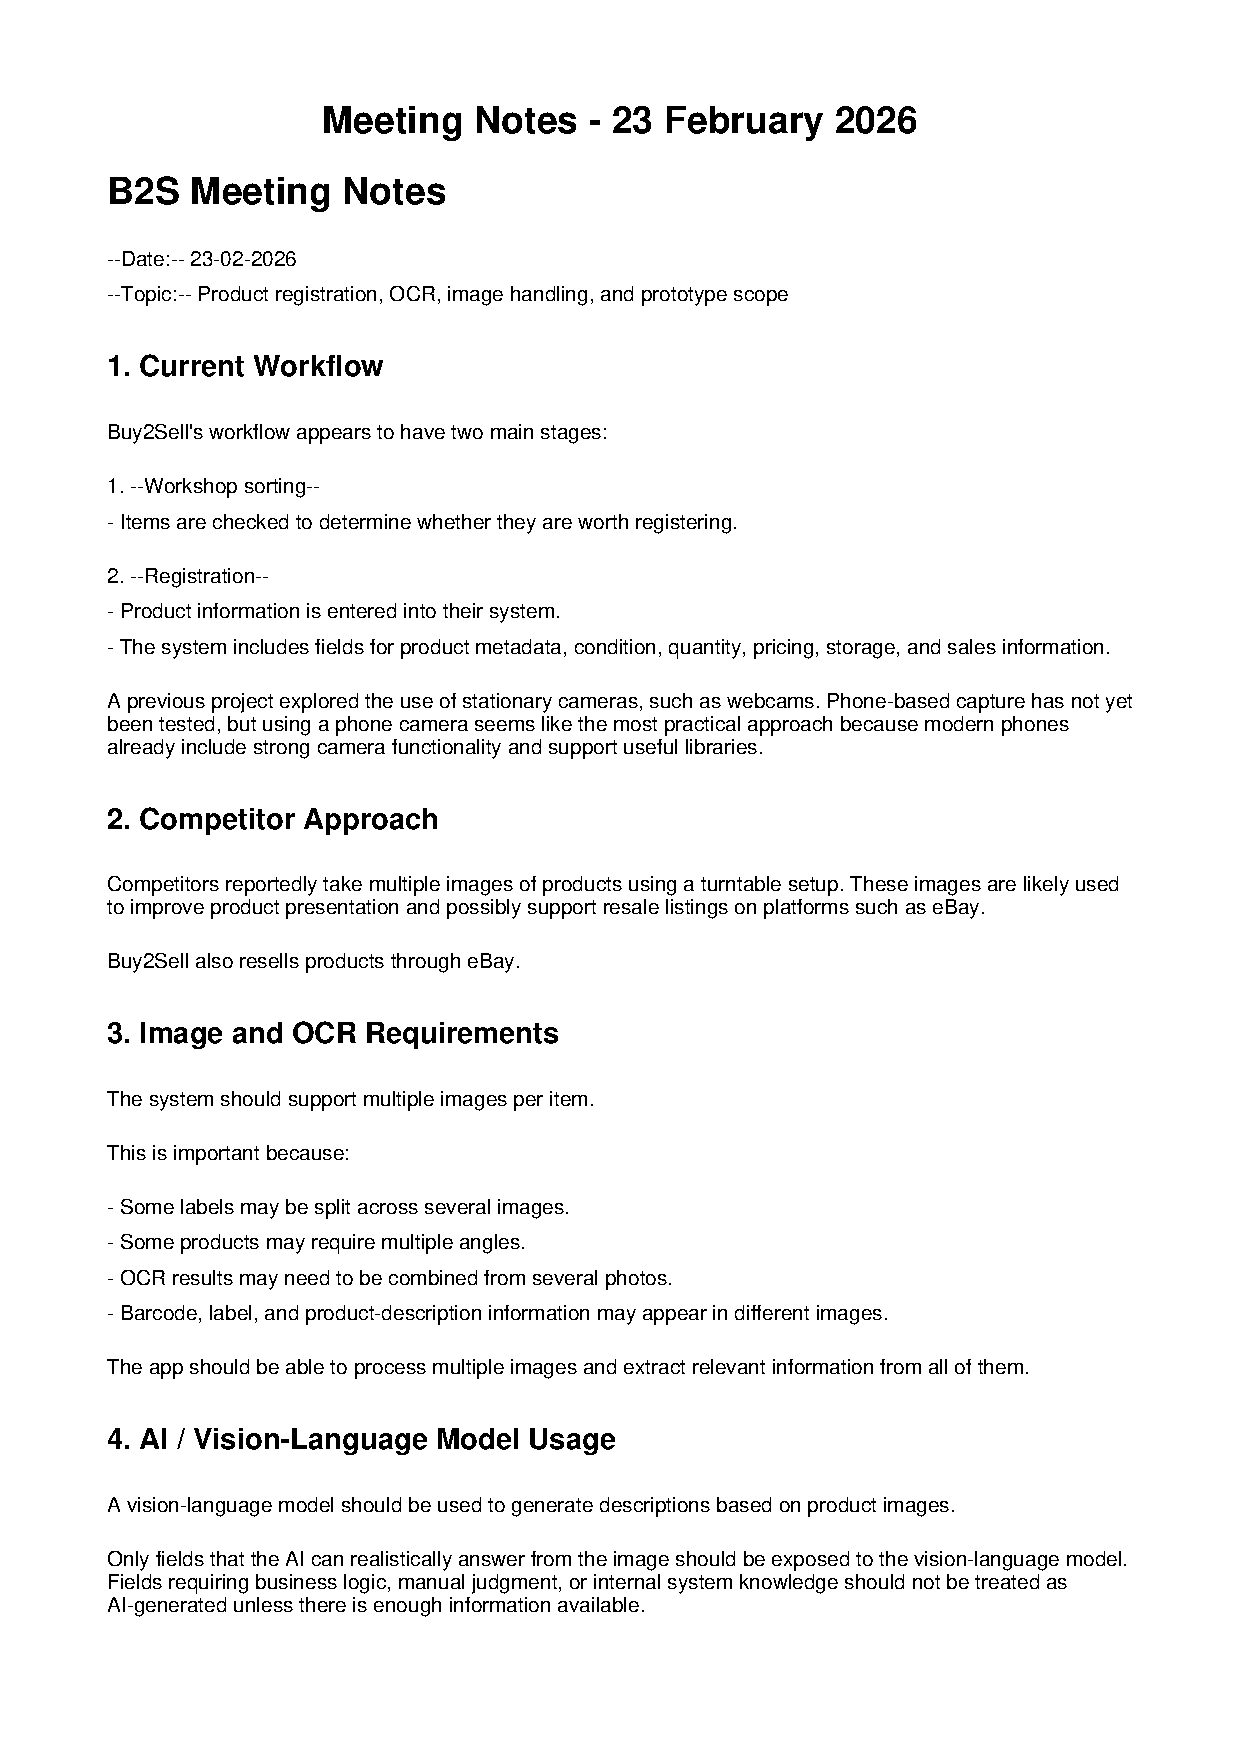
\includepdf[pages=-,pagecommand={}]{artifacts/meeting-notes-2026-02-23.pdf}
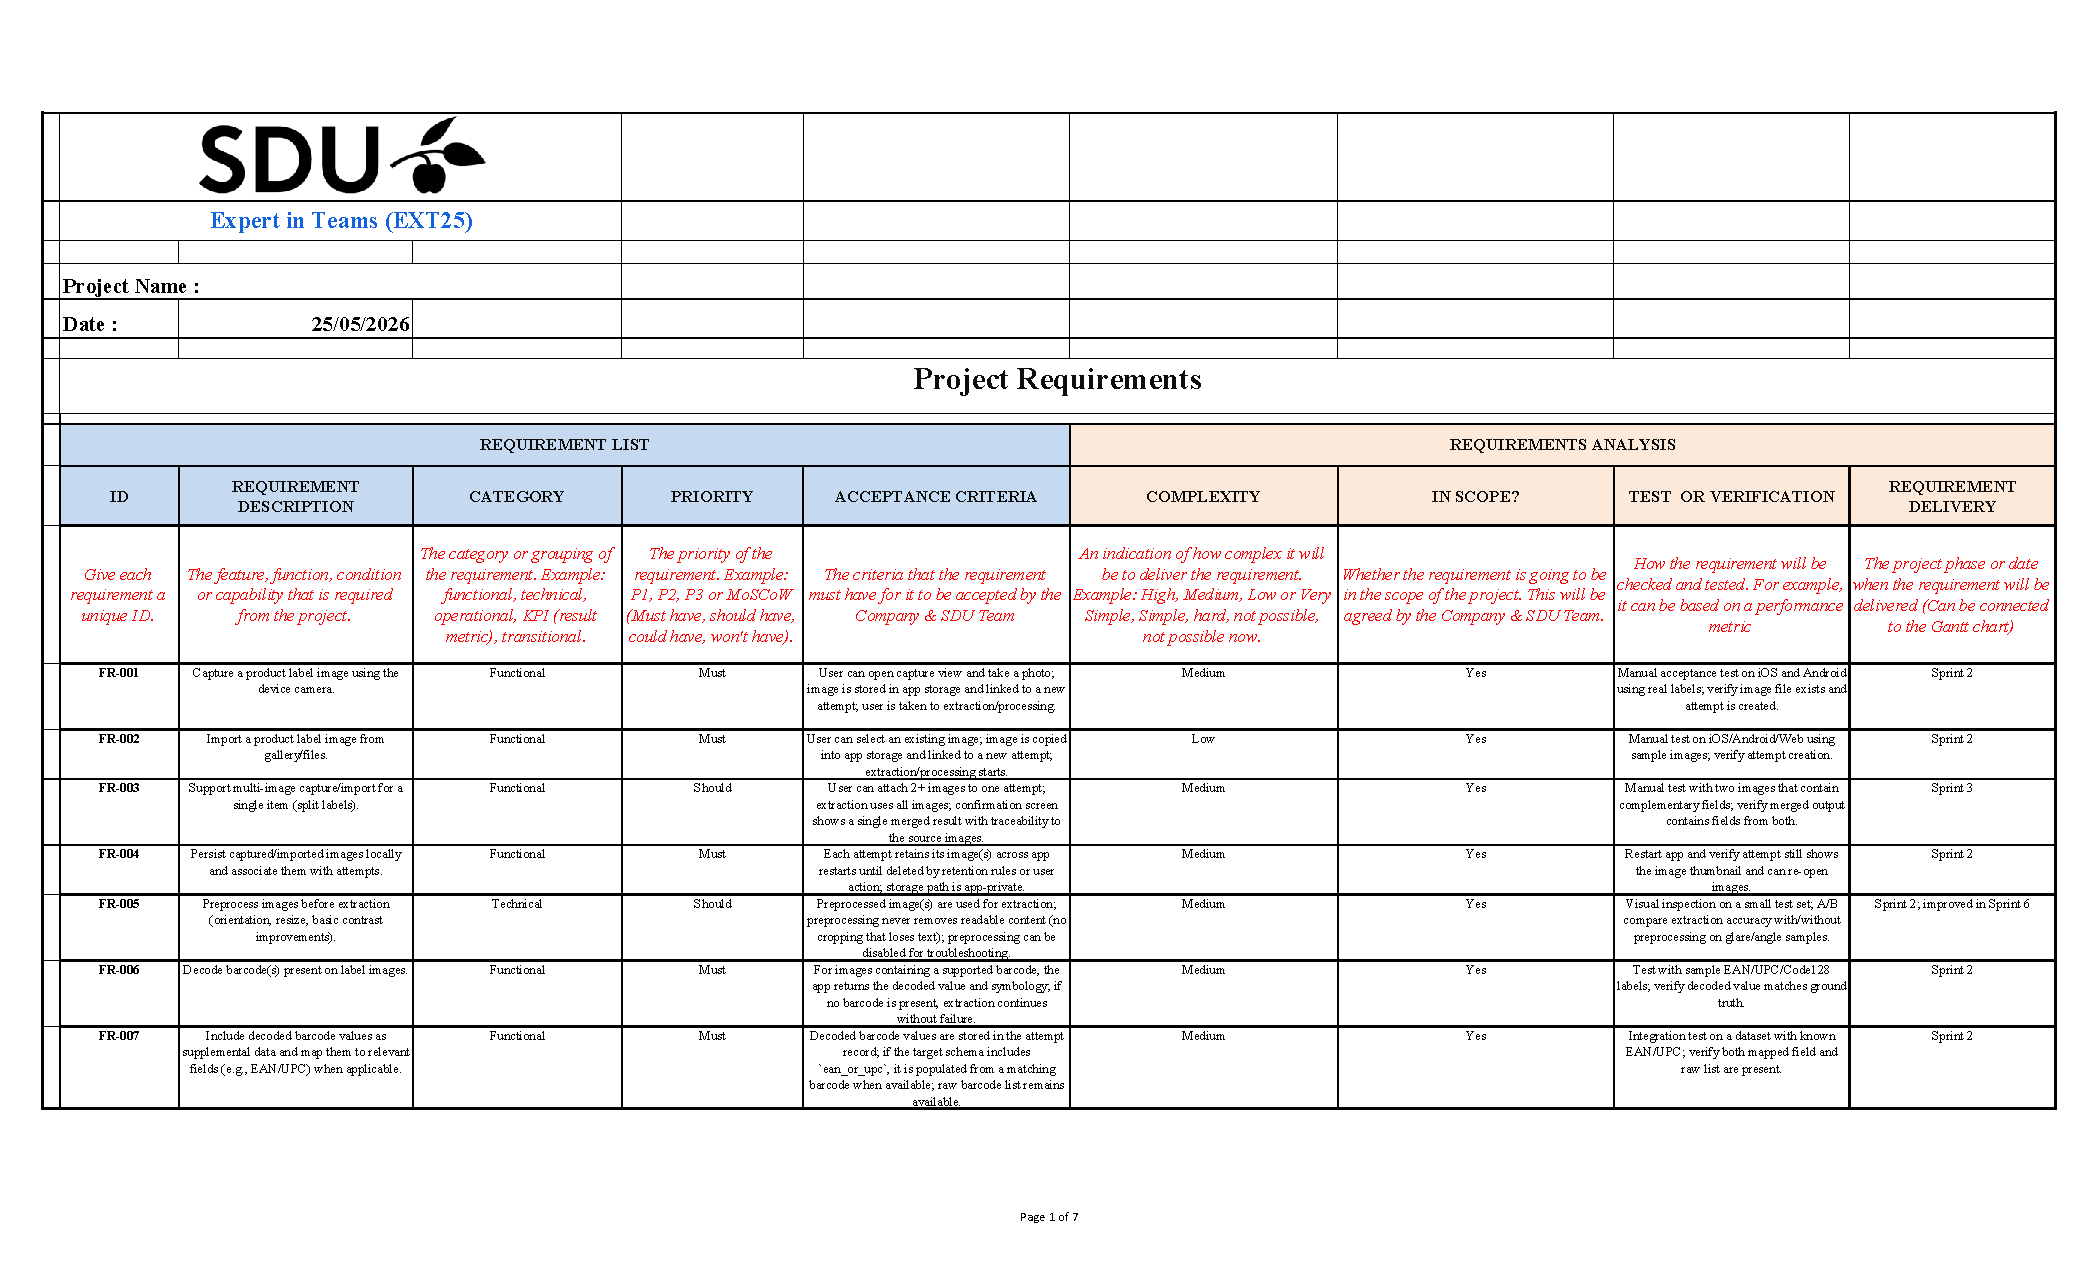
\includepdf[pages=-,pagecommand={}]{artifacts/project-requirements.pdf}
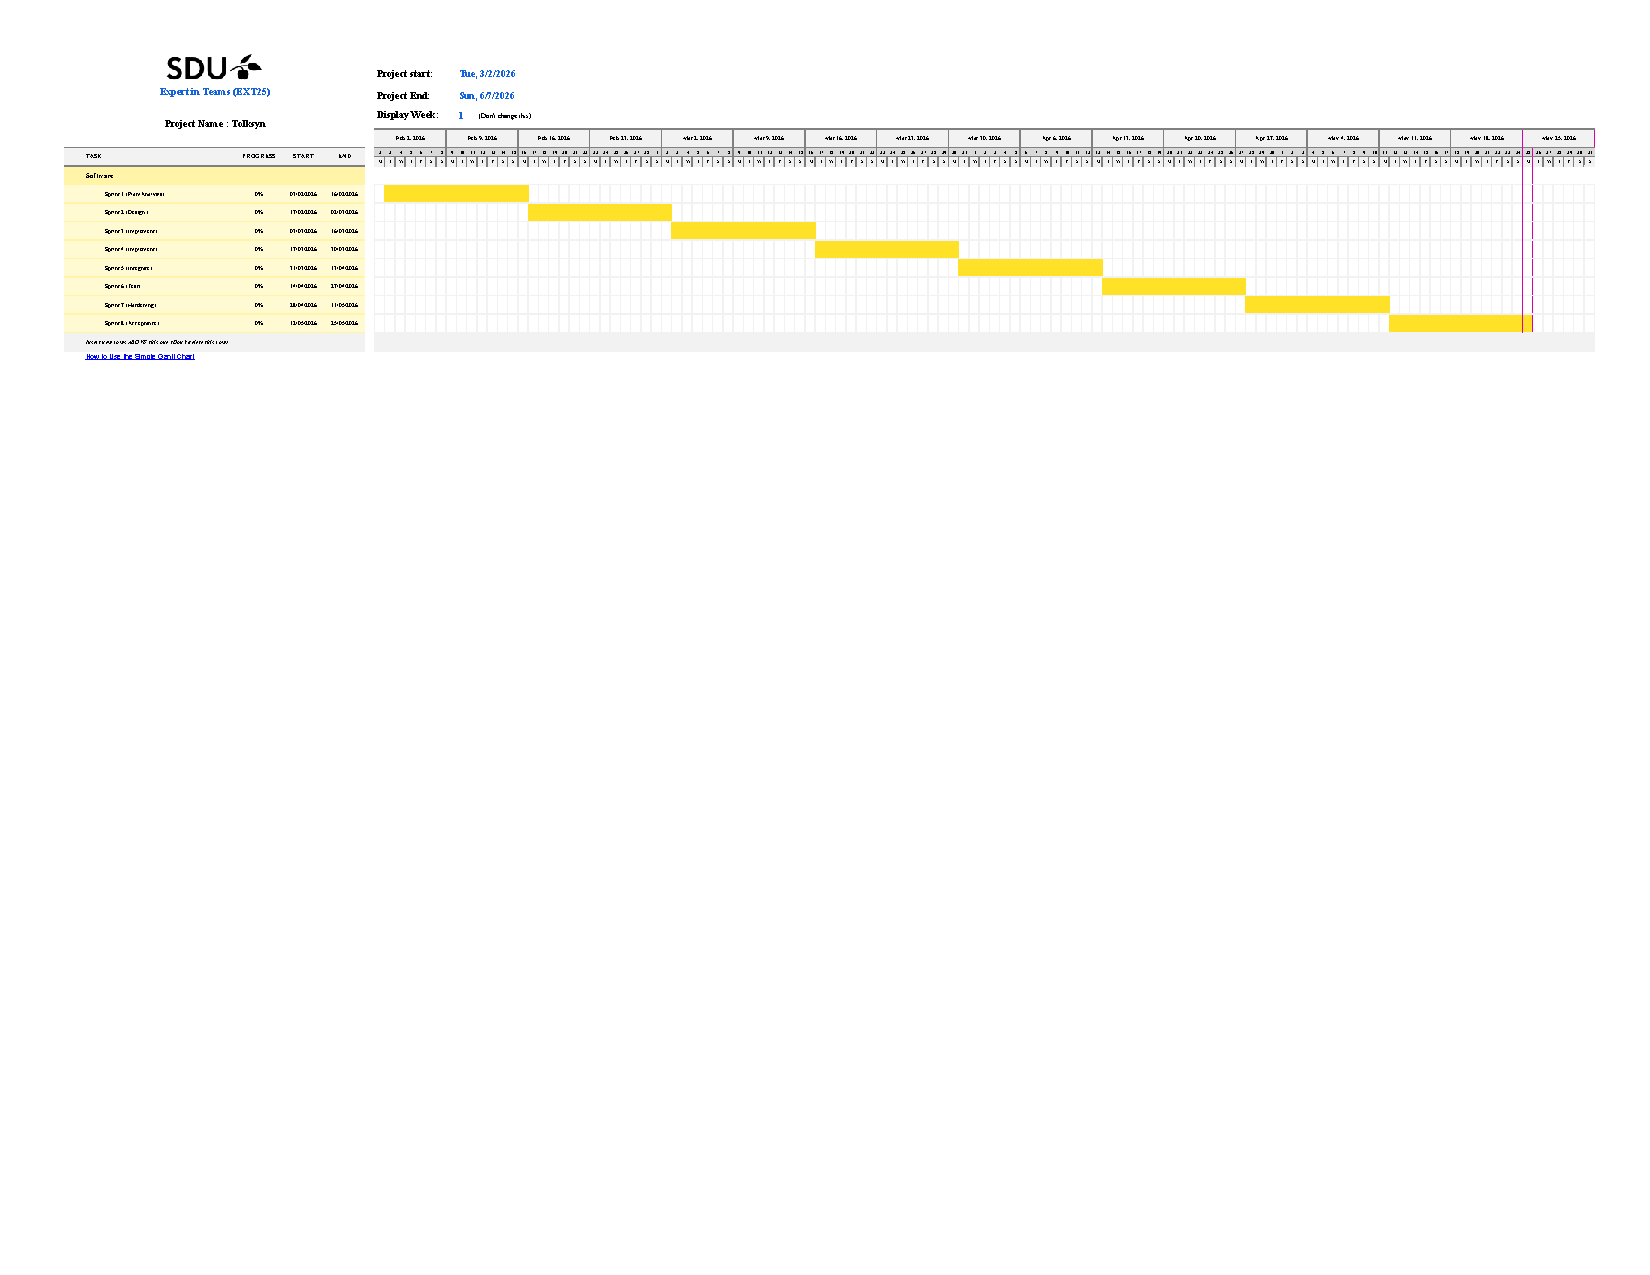
\includepdf[pages=-,pagecommand={}]{artifacts/gantt-chart.pdf}
% removed expo-app-folder-structure-best-practices.pdf
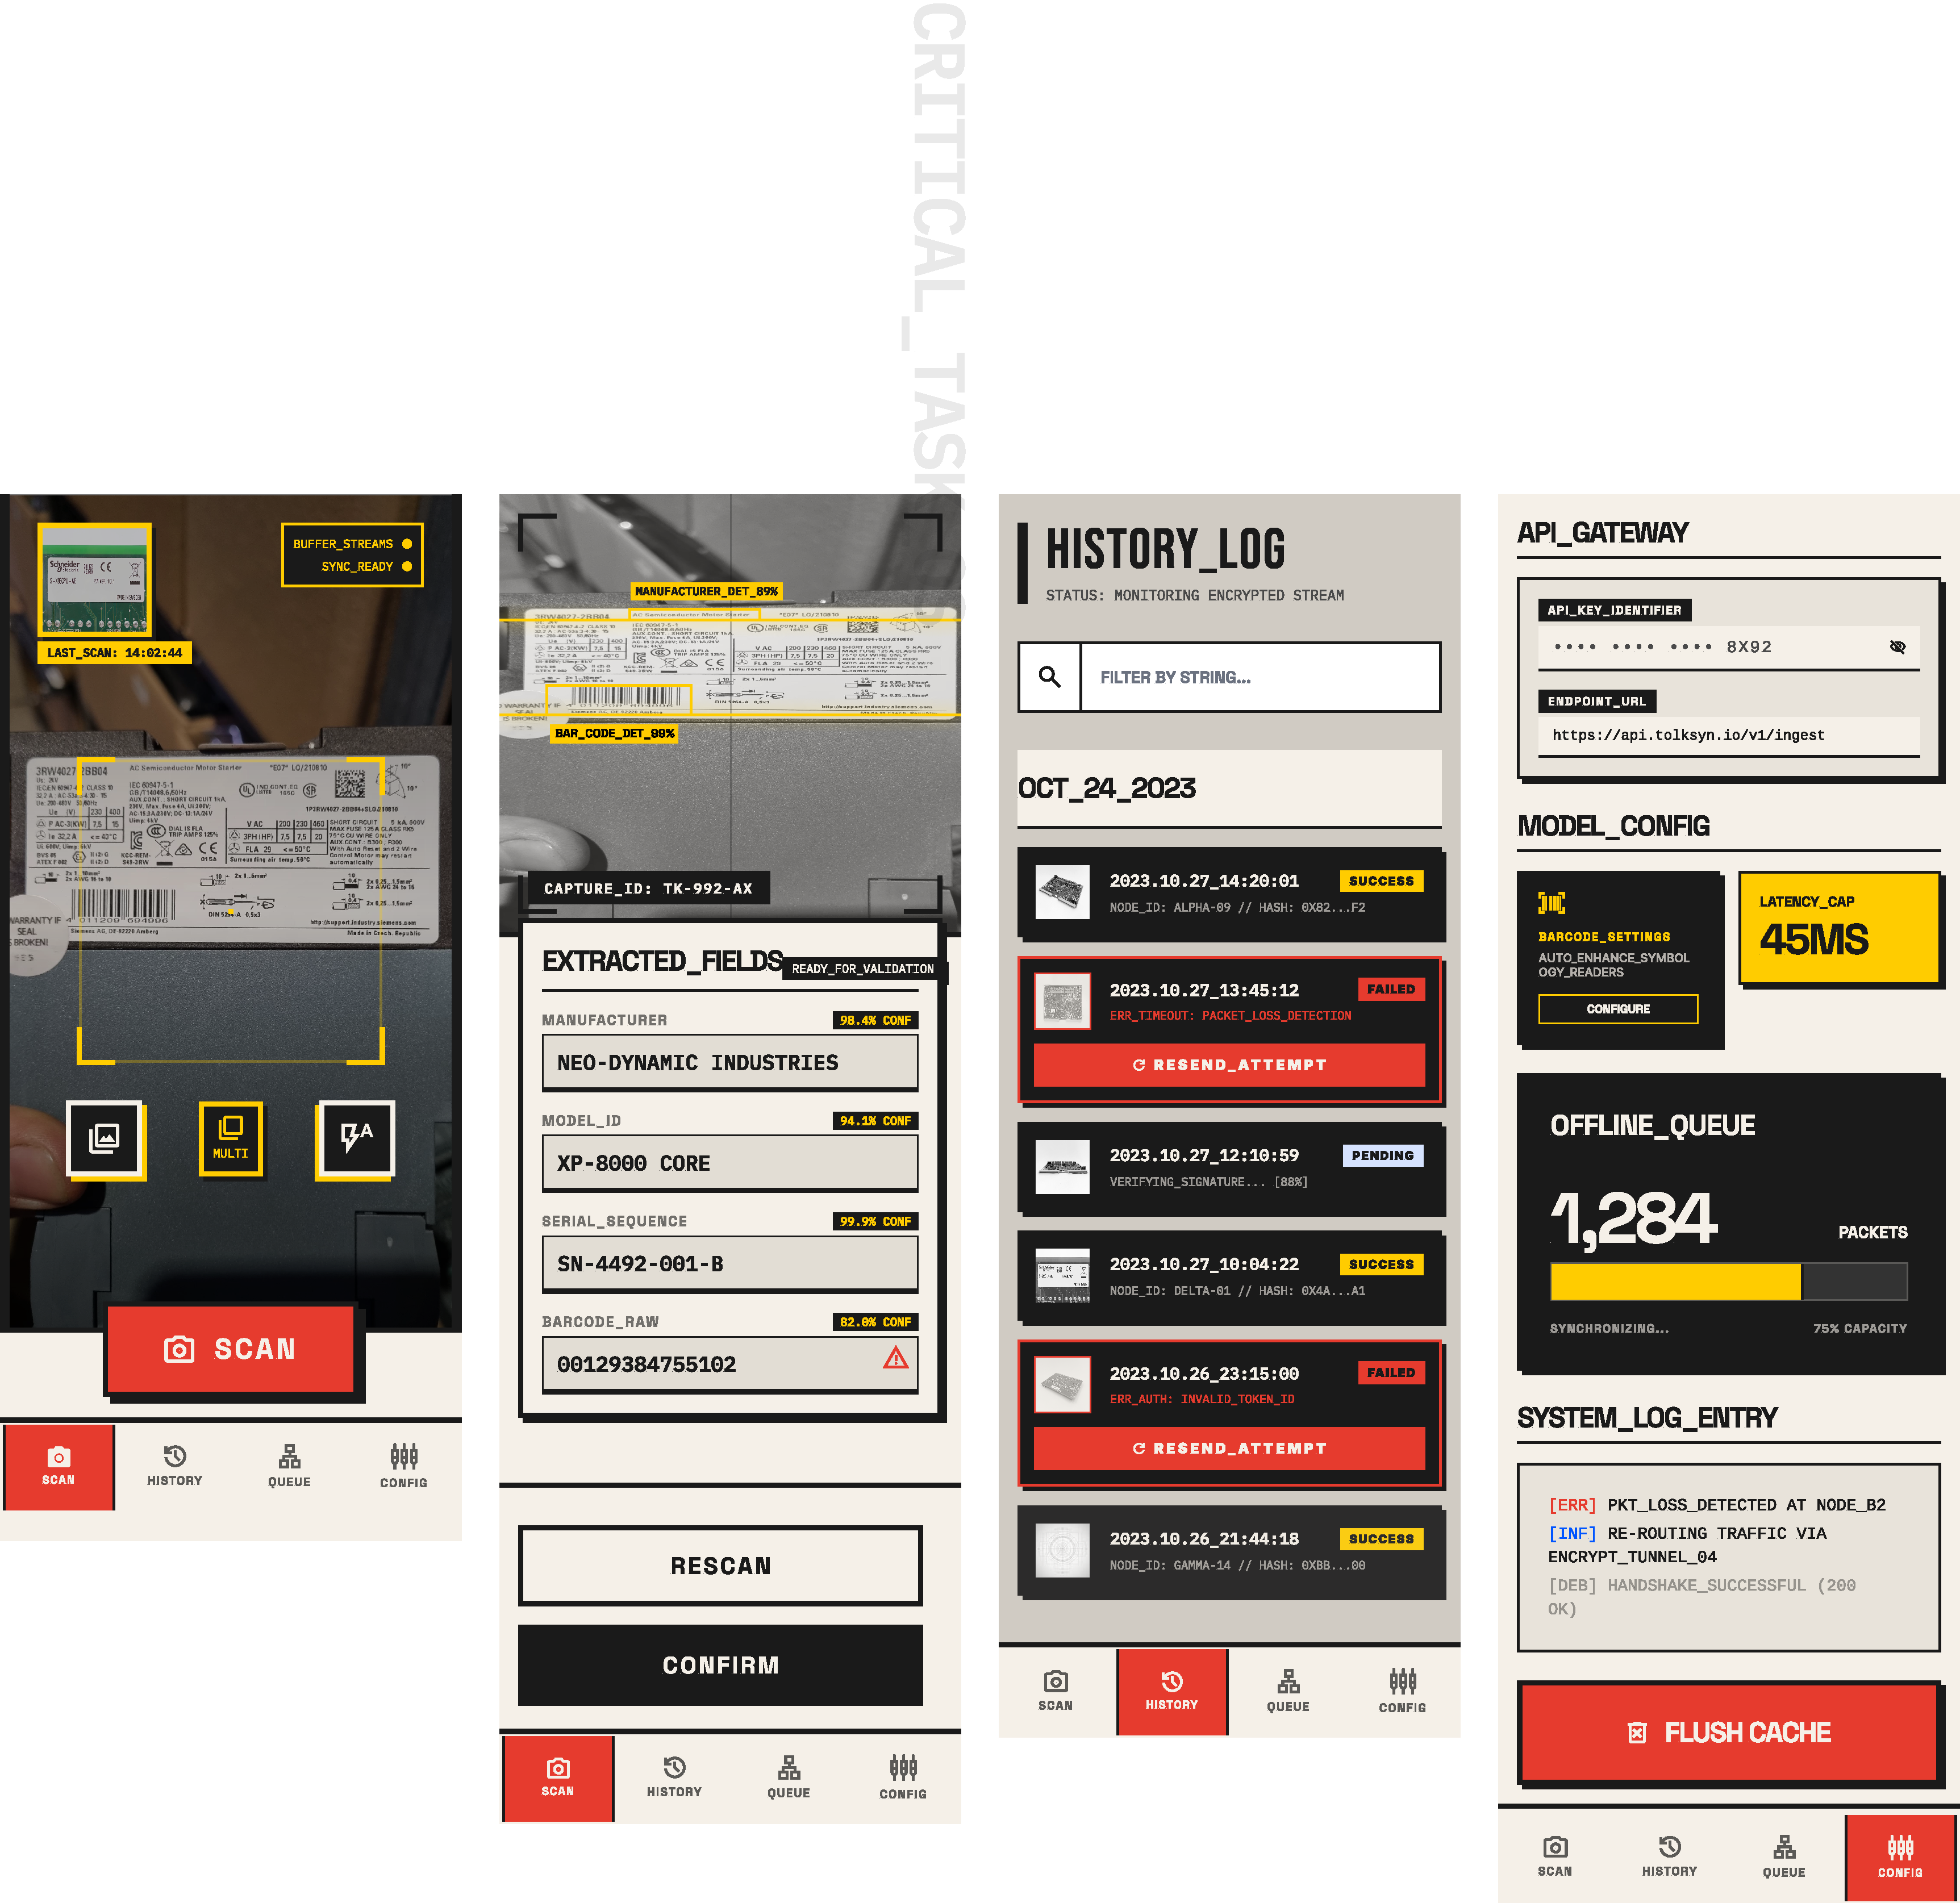
\includepdf[pages=-,pagecommand={}]{artifacts/figma-design.pdf}
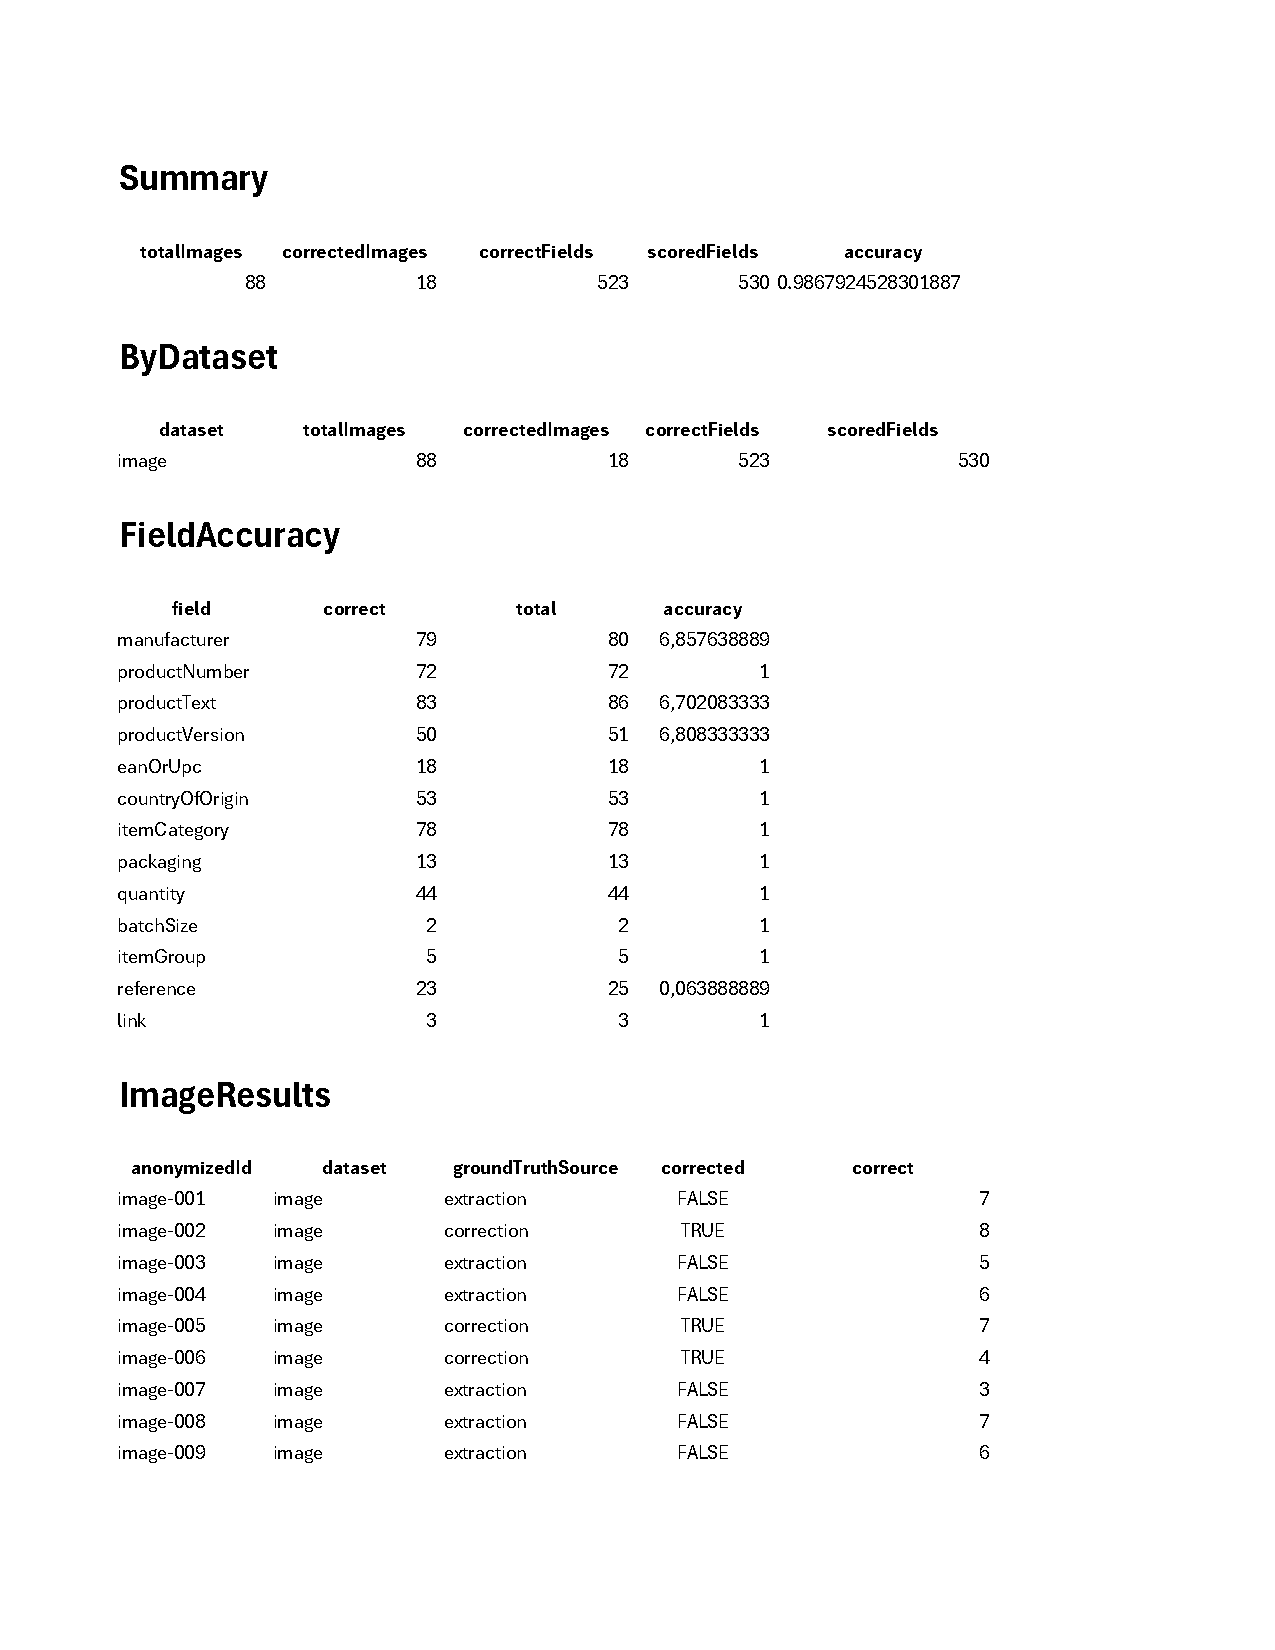
\includepdf[pages=-,pagecommand={}]{artifacts/kpi-anonymized.pdf}
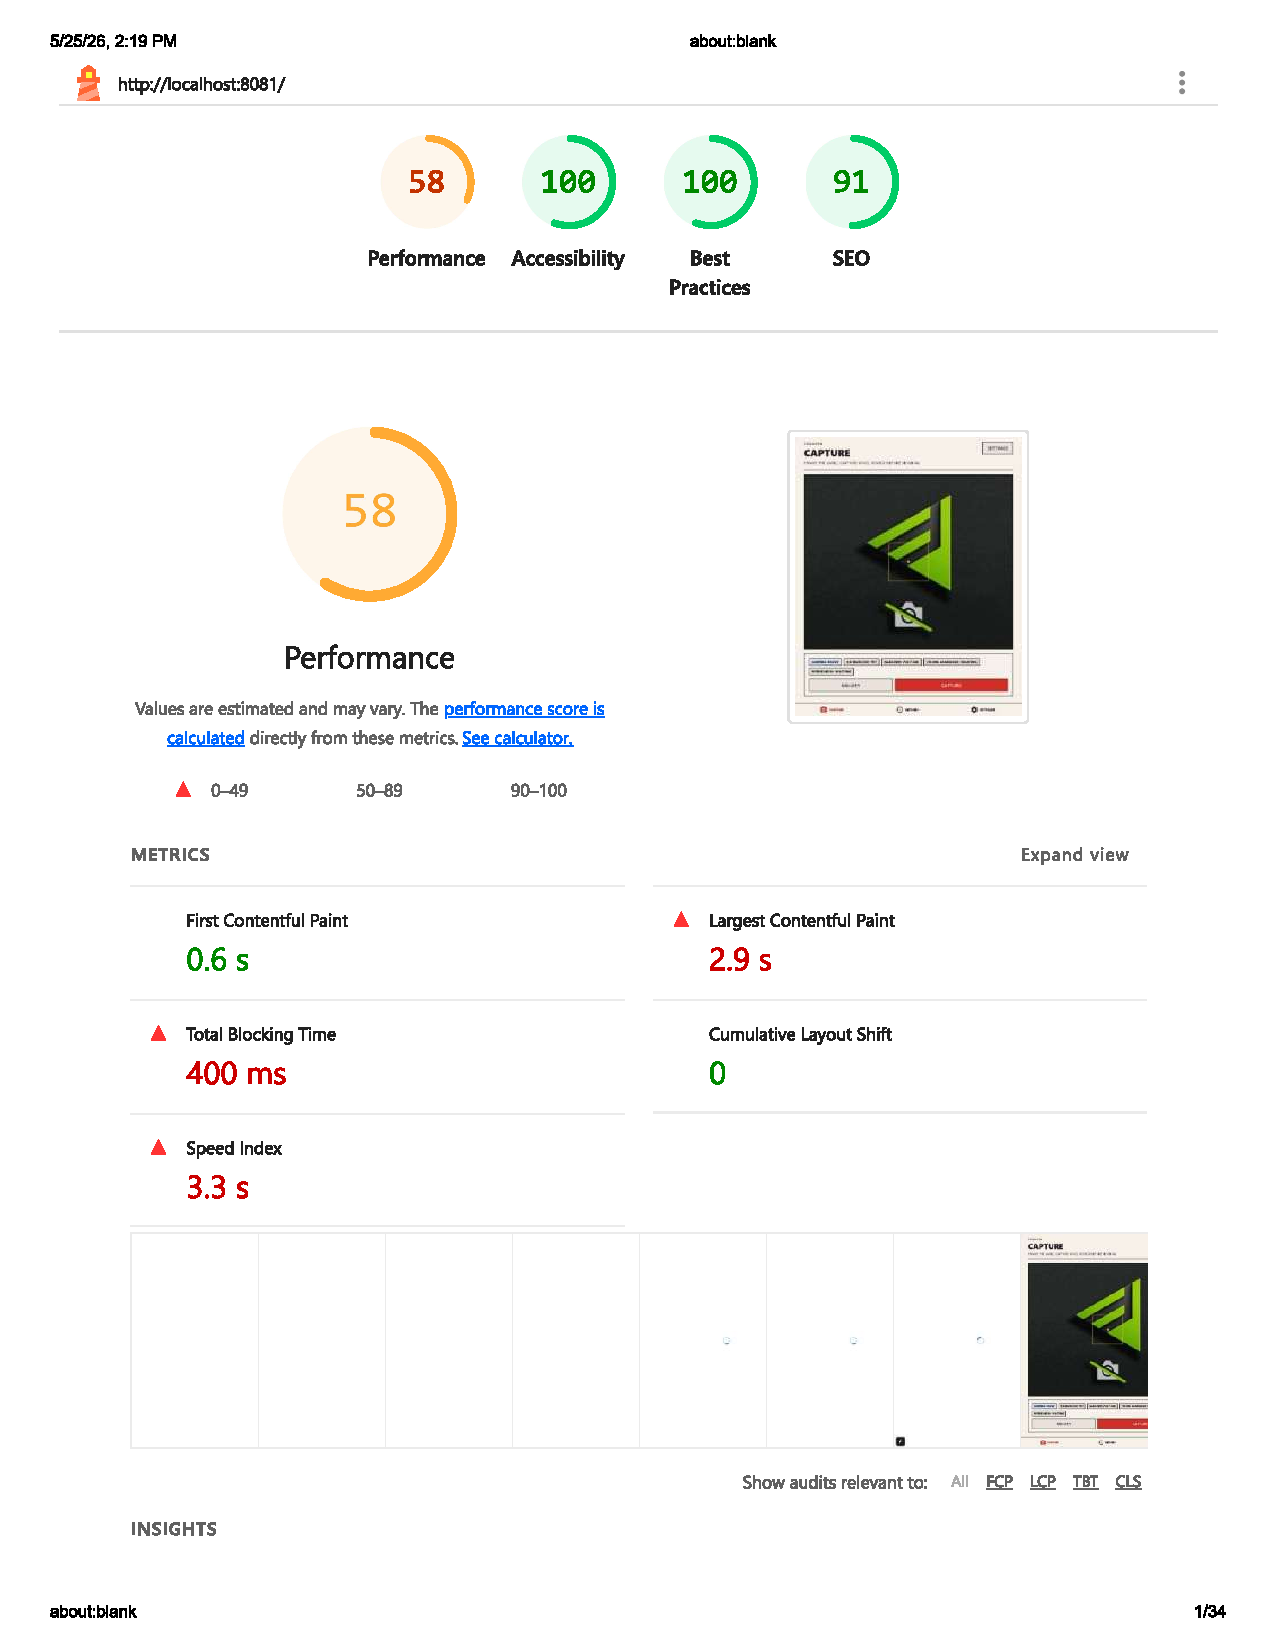
\includepdf[pages=1,pagecommand={}]{artifacts/lighthouse-capture.pdf}
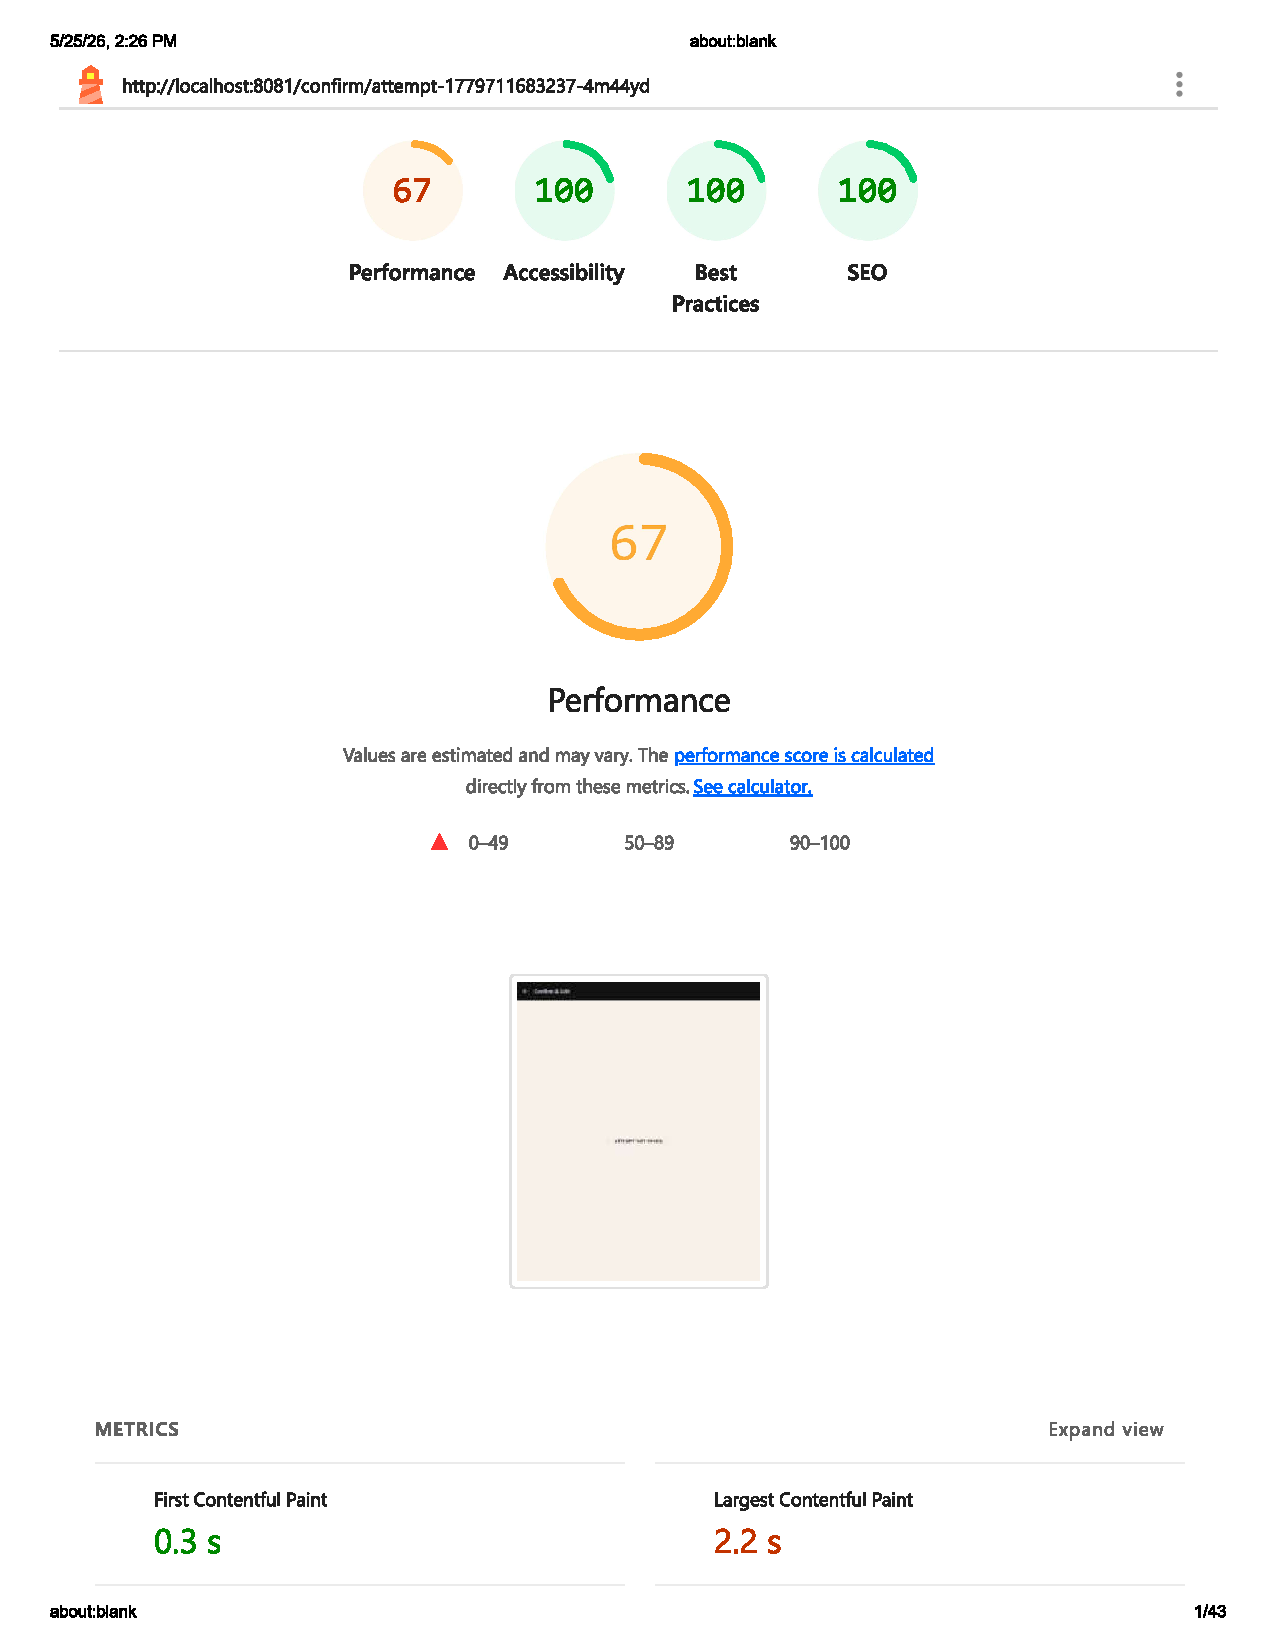
\includepdf[pages=1,pagecommand={}]{artifacts/lighthouse-confirm.pdf}
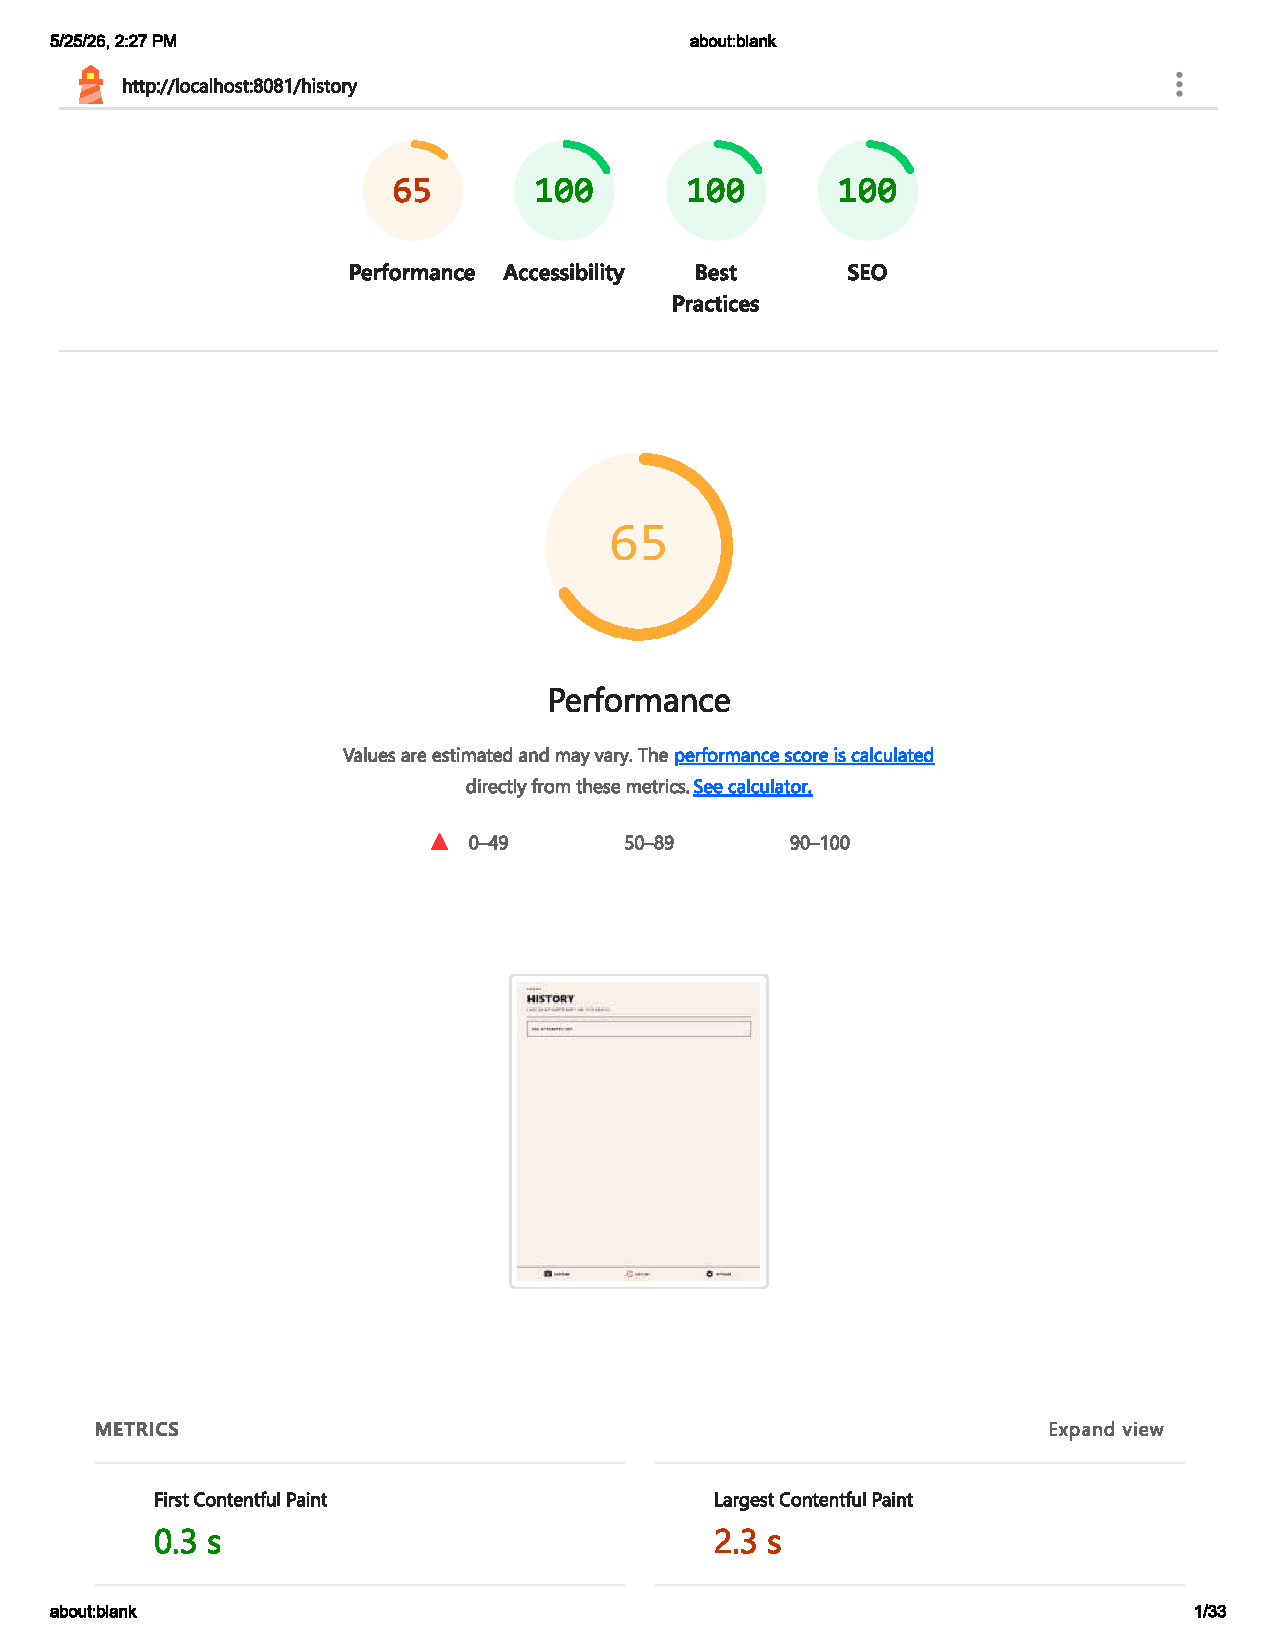
\includepdf[pages=1,pagecommand={}]{artifacts/lighthouse-history.pdf}
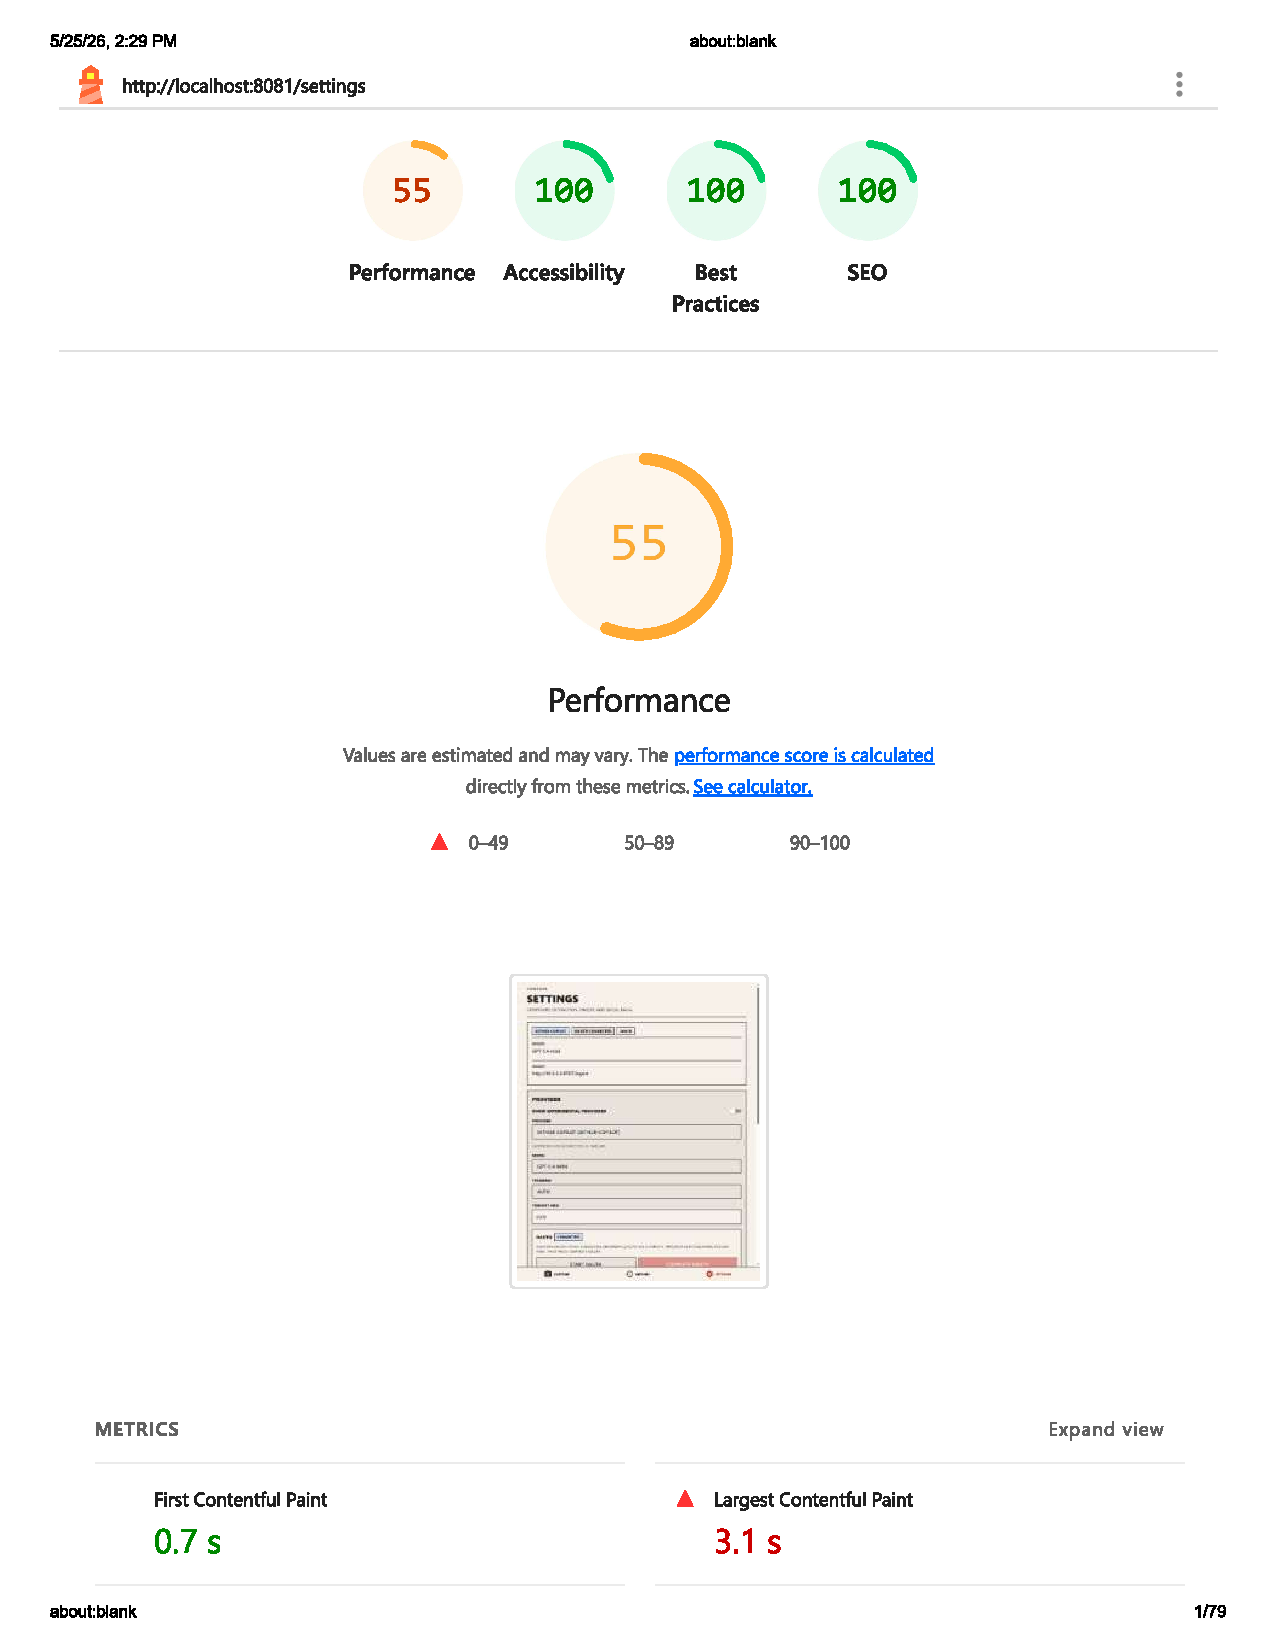
\includepdf[pages=1,pagecommand={}]{artifacts/lighthouse-settings.pdf}
